% Compile with tectonic (or pdfLaTeX twice). Style follows slides_main.tex.
\documentclass[10pt, aspectratio=169]{beamer}

\usepackage[T1]{fontenc}
\usepackage{lmodern}
\renewcommand{\familydefault}{\sfdefault}
\usepackage{amsmath, amssymb}
\usepackage{booktabs}
\usepackage{array}
\usepackage{xcolor}
\usepackage{tikz}
\usetikzlibrary{positioning, arrows.meta}

\usetheme{default}
\useinnertheme{rectangles}
\setbeamertemplate{navigation symbols}{}

\definecolor{accent}{HTML}{1A4789}
\definecolor{accent2}{HTML}{2D7A55}
\definecolor{warn}{HTML}{B8001F}
\definecolor{boxbg}{HTML}{F4F6F8}
\newcommand{\g}[1]{\textcolor{accent2}{\textbf{#1}}}
\newcommand{\bad}[1]{\textcolor{warn}{#1}}

\setbeamertemplate{itemize item}{\textcolor{accent}{\(\blacktriangleright\)}}
\setbeamertemplate{itemize subitem}{\textcolor{accent}{\(\triangleright\)}}
\setbeamercolor{frametitle}{fg=accent}
\setbeamercolor{structure}{fg=accent}
\setbeamercolor{block title}{fg=white, bg=accent}
\setbeamercolor{block body}{bg=boxbg}
\setbeamerfont{frametitle}{size=\large, series=\bfseries}

\setbeamertemplate{frametitle}{%
  \vskip0.3em%
  \begin{beamercolorbox}[wd=\paperwidth,leftskip=0.5cm,rightskip=0.5cm]{frametitle}%
    \usebeamerfont{frametitle}\insertframetitle\par%
    {\color{accent}\rule{\dimexpr\paperwidth-1cm\relax}{0.6pt}}%
  \end{beamercolorbox}%
  \vskip0.3em%
}
\setbeamertemplate{footline}{%
  \hfill\textcolor{gray}{\insertframenumber\,/\,\inserttotalframenumber}%
  \hspace{0.3cm}\vspace{0.12cm}%
}

\begin{document}

% ---------------------------------------------------------------- 1
\begin{frame}{What is being predicted, and from what}
\footnotesize
\begin{columns}[t]
\begin{column}{0.54\textwidth}
\textbf{An agent episode.} A language model drives an environment in a loop:
write an action, read what came back, write the next one --- a robot in
ALFWorld, a bash session repairing a repository in DeepSWE, a desktop in
OSWorld. It ends when the model declares it done or a step cap cuts it off,
and only then does a grader say whether the task was solved.

\smallskip
\textbf{The problem.} That verdict arrives too late to act on. While the
episode runs we want to know whether it is going anywhere --- to continue, call
a human, or stop. The input is a \emph{prefix}: the transcript up to step $k$.

\smallskip
\textbf{Why it is not trivial.} The answer depends on what has not happened
yet; the same opening steps precede either outcome. Hindsight is easy, and much
published work quietly uses it.

\smallskip
\textbf{One episode, many examples.} Truncating at every step turns one episode
into dozens of prefixes, each carrying its final outcome as the label --- where
the volume comes from, and where the leak lurks.
\end{column}
\begin{column}{0.44\textwidth}
\begin{center}
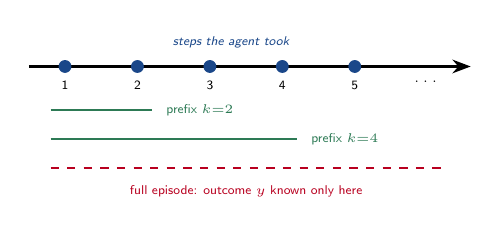
\begin{tikzpicture}[font=\tiny, >=Stealth, scale=0.92, every node/.style={scale=0.92}]
  \draw[->, thick] (0,0) -- (6.1,0);
  \foreach \x/\l in {0.5/1, 1.5/2, 2.5/3, 3.5/4, 4.5/5} {
    \filldraw[accent] (\x,0) circle (2.3pt);
    \node[below=2pt] at (\x,0) {\l};
  }
  \node[below=2pt] at (5.5,0) {$\dots$};
  \node[above=1pt, accent] at (2.8,0.1) {\textit{steps the agent took}};
  \draw[accent2, thick] (0.3,-0.60) -- (1.7,-0.60);
  \node[right=2pt, accent2] at (1.7,-0.60) {prefix $k{=}2$};
  \draw[accent2, thick] (0.3,-1.00) -- (3.7,-1.00);
  \node[right=2pt, accent2] at (3.7,-1.00) {prefix $k{=}4$};
  \draw[warn, thick, dashed] (0.3,-1.40) -- (5.8,-1.40);
  \node[warn] at (3.0,-1.72) {full episode: outcome $y$ known only here};
\end{tikzpicture}
\end{center}
\vspace{-4pt}
\vspace{-6pt}
\begin{block}{Data}
91\,279 prefixes over 18\,490 episodes in \textbf{12 cohorts} --- one cohort is
one environment $\times$ scaffold $\times$ driving model: ALFWorld
(RG/SG/RQ/SQ), DeepSWE (DG/DL/DQ), OSWorld (OQ), four code benchmarks. Labels
are binary success; DG/DL/DQ/OQ instead carry a graded \texttt{score}.
\end{block}
\vspace{-3pt}
\textbf{Model.} Qwen3.5-2B frozen, LoRA $r{=}16$ on $q,k,v,o$: 1.47\,M of
2.21\,B trainable (0.067\,\%). Prefix as text, truncated \emph{from the left}
to 2048 tokens so the question survives; last-token pooling, MLP head.
\end{column}
\end{columns}
\end{frame}

% ---------------------------------------------------------------- 2
\begin{frame}{The supervised recipe, and the number it has to beat}
\footnotesize
\begin{columns}[t]
\begin{column}{0.52\textwidth}
\textbf{What the head is trained on.} Four terms, with $y$ the episode outcome,
$p$ the head's probability and $q$ the posterior of a Bayesian tool-critic
teacher that scores the same prefix:
\[\textstyle
\mathcal{L}=\underbrace{\mathrm{BCE}(p,y)}_{\text{ranking}}
+\underbrace{(p-y)^2}_{\text{calibration}}
+\underbrace{(p-q)^2}_{\text{distillation}}
+0.3\,\underbrace{\mathcal{L}_{\text{struct}}}_{\text{repeat/stall flags}}
\]

\medskip
\textbf{Folds are cut by task, then expanded to prefixes.} Never by prefix: a
single episode yields dozens of near-identical rows, and splitting them across
the boundary puts the evaluation episode into training. One task can also
appear as up to 62 arm-level episodes, so grouping by episode is not enough
either.

\medskip
\textbf{How it is scored.} AUROC on held-out folds --- given one successful and
one failed episode, how often is the successful one ranked higher --- plus
Brier against a constant base-rate predictor, which is the honest reference for
calibration.
\end{column}
\begin{column}{0.46\textwidth}
\begin{block}{The baseline that decides everything}
Chance is not $0.50$ here. \textbf{Counting the agent's steps} already ranks
episodes: the longer it struggles, the likelier it fails.

\medskip
Two independent estimates agree:
\begin{itemize}\itemsep1pt
  \item label-permutation control, 5 folds: \g{.581}
  \item direct length baseline, same rows: \g{.581}
\end{itemize}

\medskip
\bad{Every AUROC in this work must be read against $\approx.58$, not $.50$.}
\end{block}

\smallskip
The control permutes labels \emph{inside length terciles} on purpose: that
keeps the prefix-weighted positive rate comparable, and as a side effect
preserves the length--outcome link. So it measures exactly ``signal beyond
coarse episode length'', which is the floor we need --- length leakage is a
recurring finding in this literature and in our own earlier numbers.
\end{column}
\end{columns}
\end{frame}

% ---------------------------------------------------------------- 3
\begin{frame}{The gate, and why it needs a policy gradient}
\footnotesize
\begin{columns}[t]
\begin{column}{0.48\textwidth}
\textbf{Exact utilities.} Episodes run to the end, so every action's payoff on
every prefix is \emph{known}, not estimated ($k$ = prefix step, $n$ = episode
length, $y$ = outcome):
\[
\begin{aligned}
U_{\text{cont}} &= y - c_{\text{step}}\,n\\
U_{\text{ask}}  &= 1 - c_{\text{step}}(k{+}1) - c_{\text{ask}}\\
U_{\text{stop}} &= -\,c_{\text{step}}(k{+}1)
\end{aligned}
\qquad
c_{\text{step}}=\frac{\kappa}{\mathrm{median}(n)}
\]
The step price is horizon-normalised: one constant would mean different things
in a 10-step and a 130-step environment.

\medskip
\bad{Structural caveat.} $U_{\text{ask}}-U_{\text{stop}}=1-c_{\text{ask}}$ on
\emph{every} prefix, so one dominates everywhere: at fixed costs the
three-action gate is a two-action gate. A genuine halt needs the human priced
above the task; hence $\tau_{\text{stop}}=0$.

\medskip
\textbf{Why a gradient at all.} We ship a number and the deployment reads the
action off it with a threshold: a step function, zero gradient almost
everywhere. A proper scoring rule on $p$ is then a proxy for the decision
rather than the decision.
\end{column}
\begin{column}{0.50\textwidth}
\textbf{GRPO over the confidence head.} One sigmoid becomes a categorical over
21 bins $v_j=j/20$. Sampling is free --- one forward gives the whole
distribution --- so a group of $G{=}8$ costs one supervised step.
\setlength{\abovedisplayskip}{3pt}\setlength{\belowdisplayskip}{3pt}
\[
r(x,v)=U\big(a(v),x\big)+w_{\text{cal}}\big(1-(v-y)^2\big)
\]
\[
A_{i,g}=r_{i,g}-\tfrac{1}{G}\textstyle\sum_{g'}r_{i,g'}
\]
\[
\mathcal{L}=-\overline{A_{i,g}\log\pi_\theta(j_{i,g}\mid x_i)}
            -w_H\,\overline{H[\pi_\theta(\cdot\mid x_i)]}
\]
\vspace{-5pt}\begin{block}{Three deliberate departures from CALIBER}
\begin{itemize}\itemsep1pt
  \item \textbf{No $\sigma$ normalisation} of the advantage: where the policy is
        already sure the group spread is $\approx0$, and dividing turns noise
        into a huge gradient --- the collapse their ablation reports.
  \item \textbf{No KL} to a reference policy.
  \item \textbf{Reward is the realised gate utility}, not a weighted Brier in a
        reward's clothing ($w_{\text{cal}}{=}0.3$, $w_H{=}0.01$).
\end{itemize}
\end{block}
\end{column}
\end{columns}
\end{frame}

% ---------------------------------------------------------------- 4
\begin{frame}{Results: a modest, uneven gain that pooling makes robust}
\scriptsize
\begin{columns}[t]
\begin{column}{0.53\textwidth}
\textbf{Per cohort, against that cohort's own length baseline.} Out-of-fold
AUROC; code-only training vs.\ training on all 12 cohorts.
\begin{center}\renewcommand{\arraystretch}{1.05}
\begin{tabular}{lccc}
\toprule
 & code-only & 12-cohort & length \\
\midrule
BigCodeBench  & \bad{.532} & \g{.594} & .570 \\
CodeContests  & \g{.718} & .664 & .592 \\
LiveCodeBench & \g{.678} & .669 & .553 \\
SWE-bench     & \bad{.611} & \g{.646} & .602 \\
\midrule
cohorts above length & 2 / 4 & \g{4 / 4} & --- \\
\bottomrule
\end{tabular}
\end{center}
Pooling all 12 cohorts barely moves the average --- macro .653 vs.\ length
.634 --- but it removes the dependence on \emph{which} cohort you picked. That
is the argument for the pooled recipe.

\medskip
\textbf{Distillation ablation} (code cohorts, 5 folds, floor .581):
full recipe \g{.672}, no distillation .653, control .581. Brier relative to a
constant base-rate predictor: full recipe \g{+.006}, no distillation $+.037$
--- same sign on all five folds. The teacher buys honest probabilities more
than it buys ordering.
\end{column}
\begin{column}{0.45\textwidth}
\textbf{Gate arms} (DeepSWE DG+DQ, 3 folds):
\begin{center}
\begin{tabular}{lc}
\toprule
supervised & \g{.730} \\
GRPO, no supervised stage & .708 \\
GRPO on top of SFT & \emph{in flight} \\
\bottomrule
\end{tabular}
\end{center}
Fold spread $.596$--$.881$ dwarfs the $.022$ between arms: on 164 episodes no
per-fold difference is interpretable.

\medskip
\begin{block}{Two negative results worth reporting}
\textbf{Nothing transfers across environments.} Trained on DeepSWE, scored on
the nine foreign cohorts: supervised \bad{.491}, GRPO \bad{.493} --- chance ---
while counting steps gets $.692$. Across cohorts of the \emph{same} environment
(DL) both work: $.774$, $.812$. The objective does not cross that boundary; the
representation has to.

\medskip
\textbf{The learned gate is unusable off the shelf.} It advises \emph{stop} on
57\,\% of prefixes where 60\,\% of episodes succeed --- the degeneracy above,
measured.
\end{block}
\end{column}
\end{columns}
\end{frame}

\end{document}
